\documentclass[dvipsnames]{beamer}
\usepackage{graphicx}






\usepackage{hyperref}

\title{MATH 1190 \& 1210 Meeting for Week 10}
\author{Josh}
\date{16 March 2026}

\newcommand{\transition}[1]{\frame{{}\begin{center}\fbox{#1}\end{center}}}

\begin{document}

\maketitle

\section{Logistics: Pacing}

\transition{Logistics}

\frame{{Logistics}

{\bf Where are folks in the lessons right now?}

}

\frame[t]{{Logistics: Upcoming Schedule until KC3}

    \begin{itemize}
   \item week 10 of class (16 March - 20 March)
        \begin{itemize}
        \item finish lesson 14 (if needed); lesson 15 (Net Change Meaning of an Integral)
        \item Application Day 2: Texcovas Boots Company
        \end{itemize}
    \item week 11 of class (23 March - 27 March)
        \begin{itemize}
        \item lesson 16 (Properties of Integration) -- {\footnotesize\color{red} last topic on assessment 3}
        \item lesson 17 (Antiderivatives \& Indefinite Integrals)
        \end{itemize}
    \item week 12 of class (30 March - 3 April)
        \begin{itemize}
        \item lesson 18 (FTOC) 
        \item lesson 19 (Summations)
        \item KC 3 on Tuesday 31 March (can change if needed)
        \end{itemize}
    \end{itemize}
    }

\frame[t]{{Logistics: Upcoming Deadlines}

{\bf Assessment-related Logistics}
\begin{itemize}
\item exam scored by Thurs, end of day; scores released on Fri
\item exam wrapper due on Mon; regrade requests open Tues through Thurs
\end{itemize}

{\bf Miscellaneous}
\begin{itemize}
\item Pre-class for Application Day 2 - Texcovas Boot Co. in Mobius -- not H5P! 
    \begin{itemize}
    \item Please give the activity a try in Mobius, make sure everything is working. 
    \item Let me \& Jim know if there are issues. 
    \item Contact support@digitaled.com with questions about logging in/scheduling/etc.!
    \end{itemize}
\item Assessment 3
    \begin{itemize}
    \item new targets: {\color{RedOrange}A2}, {\color{RedOrange}A3}, {\color{Fuchsia}I1}, {\color{Fuchsia}I2}
    \item reassessment targets: {\color{ProcessBlue}F2}, {\color{ForestGreen}D2}, {\color{ForestGreen}D3}, {\color{RedOrange}A1}
    \item Tuesday, 31 March, 7:00 PM; 80 minutes 
    \end{itemize}
\end{itemize}

}
\section{Content}
\transition{Content}


%%%%%%%%%%%%%%%%%%%%%%%%%%%%%%%%%%%%%

\begin{frame}{Lesson 15: Net Change}

\textbf{Examples/Exercises}
\begin{itemize}
\item Velocity $v(t)$ as the rate of change of position.
\item Growth rate $w'(t)$ as the rate of change of weight.
\item Temperature change $T'(t)$ as the rate of change of temperature.
\end{itemize}

\bigskip

\textbf{Important Ideas:}
Given a rate of change, we can determine the \textbf{net change} in the quantity over time.

\[
\text{Net Change} = \text{Area under the rate curve}
\]

\bigskip

Examples:
\begin{itemize}
\item Net change in position from velocity
\item Net change in weight from growth rate
\item Net change in temperature from temperature rate
\end{itemize}

\end{frame}

%%%%%%%%%%%%%%%%%%%%%%%%%%%%%%%%%%%%%

\begin{frame}{The Definite Integral}

The \textbf{definite integral} as a measure of net change.

\[
\int_a^b f(x)\,dx
\]

\textbf{Interpretations:}

\begin{itemize}
\item Net area between the graph of $f(x)$ and the $x$-axis
\item Net change of a quantity when $f(x)$ represents a rate
\end{itemize}

\bigskip

\textbf{Units idea}

\[
(\text{rate}) \times (\text{time}) = \text{total change}
\]

Example:
\[
\int_0^4 w'(t)\,dt
\]

represents the \textbf{total change in weight} from birth to 4 weeks.

\bigskip
\end{frame}
\begin{frame}
\textbf{Key Formula:}

If $F'(x) = f(x)$ then

\[
F(b) = F(a) + \int_a^b f(x)\,dx
\]

Connects \textbf{derivatives (rates)} with \textbf{accumulated change}.

\end{frame}



%%%%%%%%%%%%%%%%%%%%%%%%%%%%%%%%%%%%%

\begin{frame}{Application Day 2: Texcovas Boot Company}

How many labor hours maximize profit.
\begin{itemize}
\item \textbf{Student will use a Profit Model:}
\[
\text{Profit} = \text{Revenue} - \text{Cost}
\]
\item \textbf{Revenue}
\[
Revenue = p \cdot Q
\]
where
\begin{itemize}
\item $p$ = price per pair of boots
\item $Q$ = quantity produced
\end{itemize}
\textbf{Production Function}
\[
Q = zL^{\alpha}
\]
\end{itemize}

\begin{itemize}
\item $L$ = labor hours
\item $z$ = productivity level
\item $\alpha$ = elasticity of labor output
\end{itemize}
\end{frame}
\begin{frame}
\textbf{Cost}

\[
Cost = wL
\]

where $w$ is the wage per labor hour.

\bigskip

\textbf{Profit Function}

\[
P(L) = pzL^{\alpha} - wL
\]

\end{frame}

%%%%%%%%%%%%%%%%%%%%%%%%%%%%%%%%%%%%%

\begin{frame}{Maximizing Profit using the process outlined in lesson 14}

To maximize profit we:

\begin{itemize}
\item Take the derivative of the profit function
\item Find critical points where $P'(L)=0$
\item Check which value gives the largest profit (using a relevant test - \textbf{Good practice for KC3 A3!})
\end{itemize}

\bigskip

\textbf{Next Students will determine the optimal labor level}

\[
L^*=\left(\frac{pz\alpha}{w}\right)^{\frac{1}{1-\alpha}}
\]

\bigskip

\textbf{Economic Interpretation}

\begin{itemize}
\item If \textbf{price $p$ increases} $\rightarrow$ optimal labor increases
\item If \textbf{productivity $z$ increases} $\rightarrow$ optimal labor increases
\item If \textbf{wages $w$ increase} $\rightarrow$ optimal labor decreases
\end{itemize}

\bigskip
\end{frame}
\begin{frame}
\textbf{Finally, they will use calculus to help decide:}

\begin{itemize}
\item how many workers to hire
\item how production changes with technology
\item which business strategies maximize profit
\end{itemize}

\end{frame}
\section{Pedagogy}

\transition{Pedagogy}
\transition{Active Learning}
\transition{And Now - An Active Learning Discussion with Susan!}
\begin{frame}
\centering
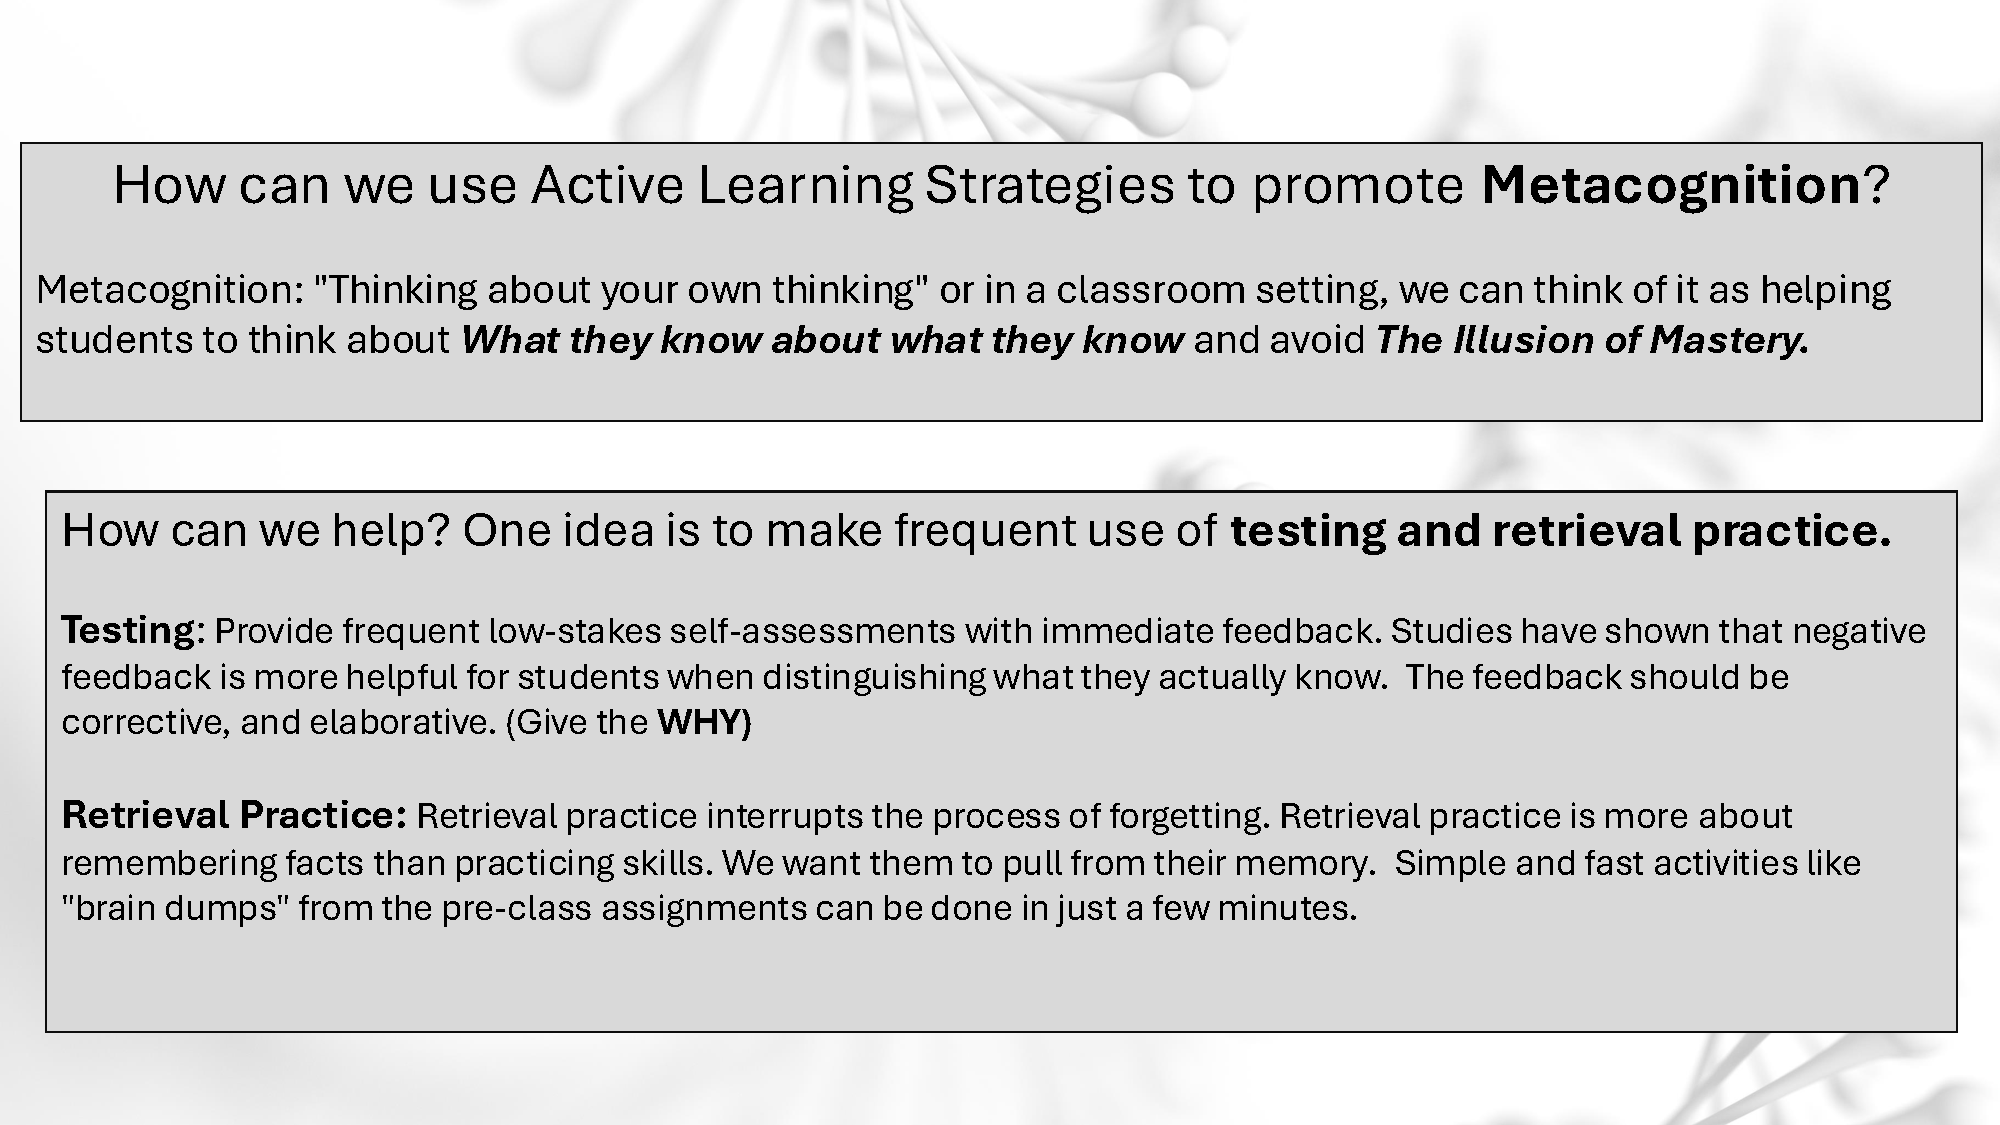
\includegraphics[width=\textwidth,page=1]{WeeklymeetingslidesSusan.pdf}
\end{frame}
\begin{frame}
\centering
\includegraphics[width=\textwidth,page=2]{WeeklymeetingslidesSusan.pdf}
\end{frame}
\begin{frame}
\centering
\includegraphics[width=\textwidth,page=3]{WeeklymeetingslidesSusan.pdf}
\end{frame}
\begin{frame}
\centering
\includegraphics[width=\textwidth,page=4]{WeeklymeetingslidesSusan.pdf}
\end{frame}
\begin{frame}
\centering
\includegraphics[width=\textwidth,page=5]{WeeklymeetingslidesSusan.pdf}
\end{frame}
\section{Renovating Calculus: A Summary of a Case Study from Augsburg University}
\vspace{6cm}

\begin{frame}{Please take a few minutes to read this summary!}
\textbf{Here is a link to the original paper:}
\vspace{0.5cm}

    \href{https://arxiv.org/pdf/2406.08508}{Renovating Calculus: A Summary of a Case Study from Augsburg University}
\end{frame}

% Slide 1: Introduction



% Slide 1: Introduction
\begin{frame}{Introduction}

\textbf{Discussion Prompt:} 
\begin{itemize}
    \item Which aspects of the study’s approach to teaching could we or do we implement in our calculus courses?
\end{itemize}
\end{frame}

% Slide 2: Teaching Strategies
\begin{frame}{Teaching Strategies Highlighted}

\textbf{Discussion Prompt:} 
\begin{itemize}
    \item Would you expect to see similar results here at UVA?
\end{itemize}
\end{frame}

% Slide 3: Assessment & Feedback
\begin{frame}{Assessment and Feedback Approaches}


\textbf{Discussion Prompt:}
\begin{itemize}
    \item How would you streamline the topics in our courses to make it more relevant to students here at UVA?
\end{itemize}
\end{frame}

% Slide 4: Curriculum Design
\begin{frame}{Curriculum Design Implications}


\textbf{Discussion Prompt:}
\begin{itemize}
    \item What curriculum adjustments could we feasibly make based on the study’s findings to better balance skills and concepts?
\end{itemize}
\end{frame}

% Slide 5: Student Engagement
\begin{frame}{Student Engagement Insights}

\textbf{Discussion Prompt:}
\begin{itemize}
    \item What are some other ways we could help students transfer their learning to new contexts?
\end{itemize}
\end{frame}

% Slide 6: Challenges and Adaptations
\begin{frame}{Challenges and Adaptations}


\textbf{Discussion Prompt:}
\begin{itemize}
    \item Which challenges might we face implementing similar strategies in our calculus curriculum, and how could we address them?
\end{itemize}
\end{frame}

% Slide 7: Takeaways
\begin{frame}{Key Takeaways}


\textbf{Discussion Prompt:}
\begin{itemize}
    \item Which one or two strategies should we prioritize testing first in our calculus courses?
\end{itemize}
\end{frame}

\end{document}


















\section{Pedagogy}

\transition{Pedagogy}

\frame[t]{{Pedagogy: Supporting Student Study Habits}

{\small

\begin{itemize}

\item Please take 7-10 minutes to read the page ``{\color{blue}\href{https://lse.ascb.org/evidence-based-teaching-guides/student-metacognition/supporting-student-learning-strategies/}{Supporting Student Learning Strategies}}".

\item Let's discuss! 
    \begin{itemize}
    \item Do the items listed in the ``What Students Do" section match your experience? Would you add any math-specific practices, or take away any listed practices?
    \item Based on what you've seen in the exam wrapper, do you feel like students do any of the practices in the ``What Students SHOULD Do" section? Where is there room for improvement?
    \item What are your thoughts on the following quote?
    \begin{center}
    {\it ``Students may avoid effective learning strategies because they cause them discomfort.  This finding suggests that students need help understanding the value of discomfort while learning."}
    \end{center}
    \end{itemize}

\item One thing that is certainly clear: students need support in using effective study practices to self-regulate their learning! The next slide contains some suggestions...

\end{itemize}
}
}

\frame{{Pedagogy: Supporting Student Study Habits}

Do you do any of the following already?

(from {\color{blue}\href{https://lse.ascb.org/wp-content/uploads/sites/10/2020/12/Instructor-Checklist_-Four-Strategies-to-Foster-Student-Metacognition.pdf}{{\bf Four Strategies to Implement in Any Course}}}
\begin{enumerate}
\item Instruct students about the power of retrieval practice for improving their retention and exam
performance.
\item Encourage students to space their practice.
\item Develop practice questions that help your students accurately monitor their learning.
\item Prompt students to develop study plans and to evaluate their approaches after an exam.
\end{enumerate}

\

How can you improve?

}

\end{document}

%%%%%%%%%%%%%%%%%%%%%%%%%%%%%

\frame[t]{{Pedagogy}

The article frames that the snowball effect as a challenge made more prominent by alternative grading systems, but not a bug: 

\

``I think this experience, where you have to move on to concept N+1 before you have fully mastered concept N, is normal in our own experiences as learners. Sometimes we can’t fully grasp a concept or topic until we move on to something higher, requiring us to put that earlier concept on the back burner for a while...The lesson here is that while the “snowball effect” might be inevitable in situations where you get more than one opportunity to demonstrate learning, and while it might be ideal for you while it happens, it’s not a critical flaw in alternative grading – it’s just a normal part of the nonlinear nature of learning things."

\

Traditional methods almost by definition do not have this snowball effect (unless you count studying for a final exam). But this is because they don’t have feedback loops. By removing the loop, you remove the snowballing. That is a partial win for students, because they never have to deal with shoring up skill on old topics while new ones are emerging; but it’s also a big loss, for the same reason. On balance, students are better off having feedback loops with the possibility of a snowball than they are without feedback loops and no snowball."

}
